Two different ways of combining the spectra of individual antennas are presented. One is combining the data in time domain by summation and calculating the spectrum afterwards and the other is combining the spectra calculated from the individual antenna data. Because of the linearity property of the fourier transform, the results or spectra of both these summations are the same (figures \ref{fig:t2-sup-mag} to \ref{fig:t2-comb-phase}).\\

The magnitudes of the spectra seem to be the same as the one of receiver channel 1 (combination) which can be seen in task 1.

\begin{figure}
    \centering
    \begin{minipage}{0.48\textwidth}
        \centering
        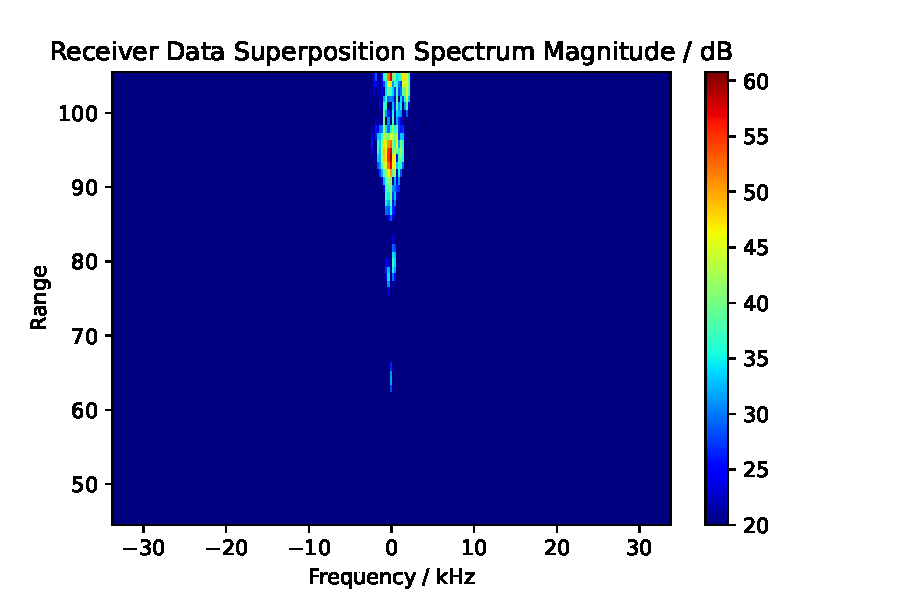
\includegraphics[width=\textwidth]{graphics/t2/t2-sup-mag.pdf}
    \caption{Task 2: Magnitude of spectrum of time series superposition of receivers 2-5.}
    \label{fig:t2-sup-mag}
    \end{minipage}\hfill
    \begin{minipage}{0.48\textwidth}
        \centering
             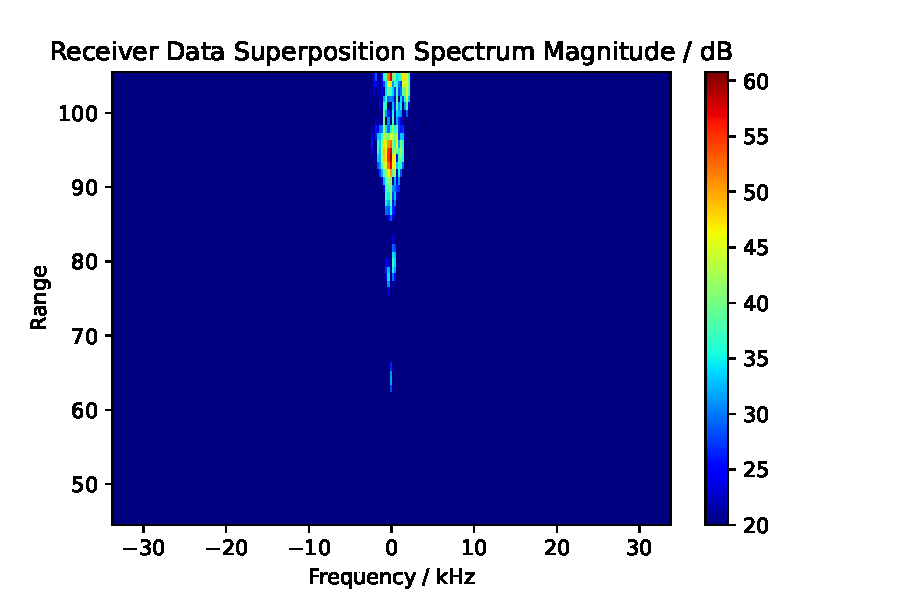
\includegraphics[width=\textwidth]{graphics/t2/t2-sup-mag.pdf}
    \caption{Task 2: Magnitude of individual spectrum combination of receivers 2-5.}
    \label{fig:t2-comb-mag}
    \end{minipage}
\end{figure}

\begin{figure}
    \centering
    \begin{minipage}{0.48\textwidth}
        \centering
        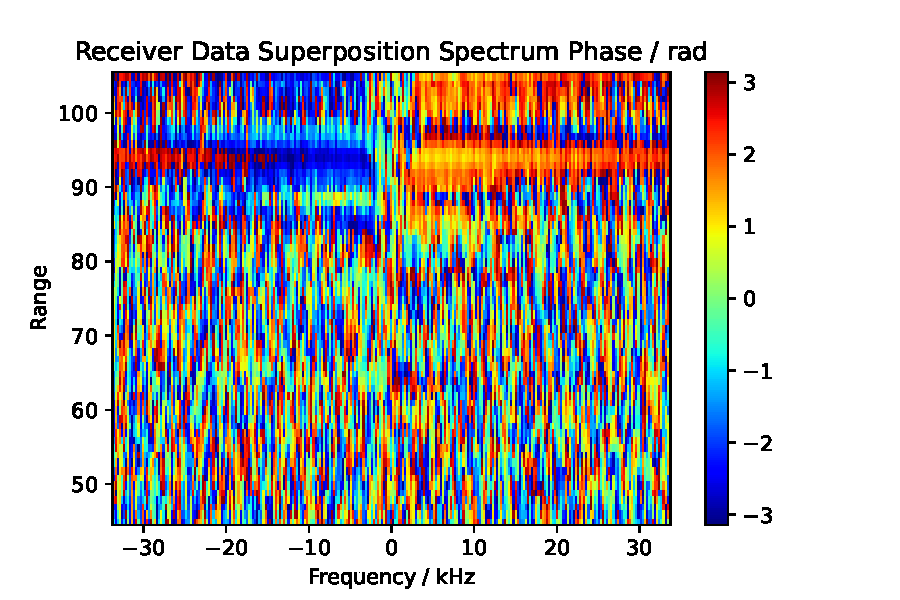
\includegraphics[width=\textwidth]{graphics/t2/t2-sup-phase.pdf}
    \caption{Task 2: Phase of spectrum of time series superposition of receivers 2-5.}
    \label{fig:t2-sup-phase}
    \end{minipage}\hfill
    \begin{minipage}{0.48\textwidth}
        \centering
        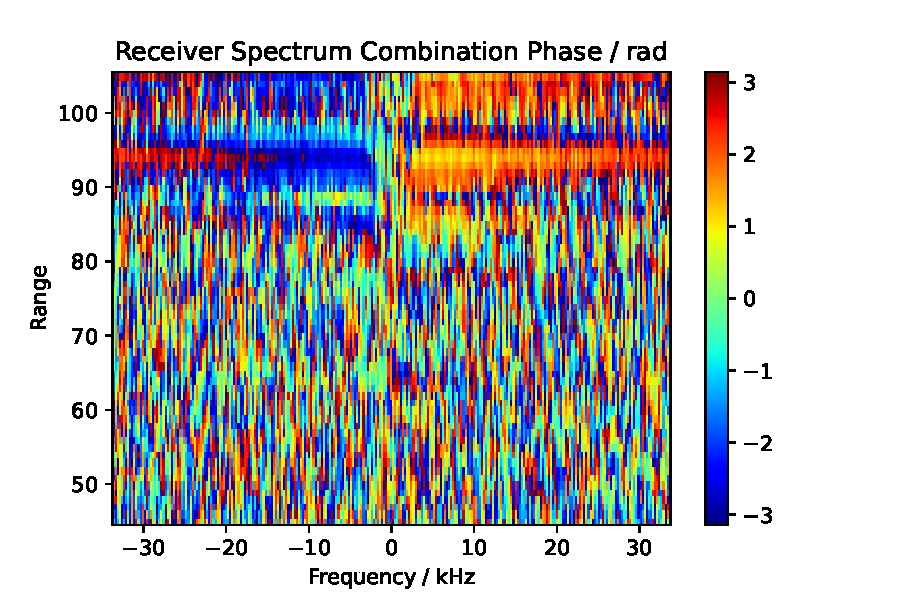
\includegraphics[width=\textwidth]{graphics/t2/t2-comb-phase.pdf}
    \caption{Task 2: Phase of individual spectrum combination of receivers 2-5.}
    \label{fig:t2-comb-phase}
    \end{minipage}
\end{figure}
